\documentclass{article}
\usepackage{amsmath,amssymb,amsthm}
\usepackage{booktabs}
\usepackage{tikz}
\usepackage{graphicx}
\usepackage{hyperref}
\usepackage{enumitem}
\usepackage{float}


\author{kipngeno koech - bkoech}
\title{Homework 3 - Introduction to Probabilistic Graphical Models}   

\date{}

\begin{document}

\maketitle

\section{Sampling (Monte-Carlo), MCMC[50 points]}

\subsection{(Monte-Carlo) [20 points]}

Given a random distribution $p(x)$ on $x = [x_1, ..., x_D]^T \in \mathbb{R}^D$. Suppose we want to perform inference
$\mathbb{E}_{p(x)}[f(x)]$ using importance sampling, with $q(x)$ as the proposal distribution. According to importance
sampling, we draw $L$ i.i.d. samples $x^{(1)}, ..., x^{(L)}$ from $q(x)$, and we have
$$\mathbb{E}_{p(x)}[f(x)] \approx \frac{1}{\sum_{i=1}^L u_i} \sum_{i=1}^L f(x^{(i)})u_i$$
where the (unnormalized) importance weights $u_i = \frac{p(x^{(i)})}{q(x^{(i)})}$.

\begin{enumerate}
\item (5 points) Find the mean and variance of the unnormalized importance weights $\mathbb{E}_{q(x)}[u_i]$ and $\mathrm{Var}_{q(x)}[u_i]$.
\[
\mathbb{E}_{q(x)}[u_i] = \int q(x) \frac{p(x)}{q(x)} dx = \int p(x) dx = 1
\]
\[
\mathrm{Var}_{q(x)}[u_i] = \int q(x) \left(\frac{p(x)}{q(x)} - 1\right)^2 dx = \int q(x) \frac{p^2(x)}{q^2(x)} dx - 1
\]

\item (5 points) Prove the following lemma: $\mathbb{E}_{p(x)}\left[\frac{p(x)}{q(x)}\right] \geq 1$, and the equality holds only when $p = q$.
\[
\mathbb{E}_{p(x)}\left[\frac{p(x)}{q(x)}\right] = \int p(x) \frac{p(x)}{q(x)} dx = \int p^2(x) \frac{1}{q(x)} dx
\]
Using Cauchy-Schwarz inequality, we have
\[
\int p^2(x) \frac{1}{q(x)} dx \geq \left(\int p(x) dx\right)^2 = 1
\]
The equality holds only when $p(x) = q(x)$.
\item (9 points) A measure of the variability of two components in vector $u = [u_1, ..., u_L]^T$ is given by
$\mathbb{E}_{q(x)}\left[(u_i - u_j)^2\right]$. Assume that both $p$ and $q$ can be factorized, i.e. $p(x) = \prod_{i=1}^D p_i(x_i)$, and $q(x) = \prod_{i=1}^D q_i(x_i)$. Show that $\mathbb{E}_{q(x)}\left[(u_i - u_j)^2\right]$ has exponential growth with respect to $D$.
\[\]
\item (1 point) Use the conclusion in (c) to explain why the standard importance sampling does not scale well
with dimensionality and would blow up in high-dimensional cases.
\end{enumerate}

\subsection{(MCMC)[40 points]}
\subsubsection{Multiple Choice [10 points]}
\begin{enumerate}
\item (5 points) Which of the following statements is true for the acceptance probability
$A(x'|x) = \min(1, \frac{P(x')Q(x|x')}{P(x)Q(x'|x)})$ of Metropolis-Hastings algorithm?
\begin{enumerate}
\item It satisfies detailed balance.
\item We can just evaluate $P(x')$ and $P(x)$ up to a normalization constant.
\item It ensures that the MH algorithm eventually converges to the true distribution.
\item All of the above.
\end{enumerate}

The correct answer is \textbf{(d)}. The acceptance probability satisfies detailed balance, we can evaluate $P(x')$ and $P(x)$ up to a normalization constant, and it ensures that the MH algorithm eventually converges to the true distribution.

\item (5 points) Which of the following statements is true for Hamiltonian Monte Carlo in comparison with
vanilla MCMC?
\begin{enumerate}
\item It can improve acceptance rate and give better mixing.
\item Stochastic variants can be used to improve performance in large dataset scenarios.
\item It may not be used for discrete variable.
\item All of the above.
\end{enumerate}
\end{enumerate}

The correct answer is \textbf{(d)}. Hamiltonian Monte Carlo can improve acceptance rate and give better mixing, stochastic variants can be used to improve performance in large dataset scenarios, and it may not be used for discrete variable.

\subsubsection{Modeling with Markov Chain Monte Carlo [30 points]}

We are going to use the data from the 2013-2014 Premier League PL1 to build a predictive model on the
number of goals scored in a single game by the two opponents. Bayesian hierarchical model is a good
candidate for this kind of modeling task. We model each team's strength (both attacking and defending) as
latent variables. Then in each game, the goals scored by the home team is a random variable conditioned
on the attacking strength of the home team and the defending strength of the away team. Similarly, the
goals scored by the away team is a random variable conditioned on the attack strength of the away team
and the defense strength of the home team. Therefore, the distribution of the scoreline of a specific game is
dependent on the relative strength between the home team A and the away team B, which also depends on
the relative strength between those teams with their other opponents.

\begin{table}[h]
\centering
\caption{2013-2014 Premier League teams}
\begin{tabular}{ccccc}
\hline
Index & 0 & 1 & 2 & 3 \\
Team & Arsenal & Aston Villa & Cardiff City & Chelsea \\
\hline
Index & 4 & 5 & 6 & 7 \\
Team & Crystal Palace & Everton & Fulham & Hull City \\
\hline
Index & 8 & 9 & 10 & 11 \\
Team & Liverpool & Manchester City & Manchester United & Newcastle United \\
\hline
Index & 12 & 13 & 14 & 15 \\
Team & Norwich City & Southampton & Stoke City & Sunderland \\
\hline
Index & 16 & 17 & 18 & 19 \\
Team & Swansea City & Tottenham Hotspur & West Bromwich Albion & West Ham United \\
\hline
\end{tabular}
\end{table}

Here we consider using the same model as described by Baio and Blangiardo. The Premier League has
20 teams, and we index them as in Table 1. Each team would play 38 matches every season (playing each of
the other 19 teams home and away), which totals 380 games in the entire season. For the $g$-th game, assume
that the index of home team is $h(g)$ and the index of the away team is $a(g)$. the observed number of goals
is:

$$y_{gj} | \theta_{gj} = \text{Poisson}(\theta_{gj})$$

where the $\theta = (\theta_{g1}, \theta_{g2})$ represent the scoring intensity in the g-th game for the team playing at home
($j = 1$) and away ($j = 2$), respectively. We put a log-linear model for the $\theta$s:

$$\log \theta_{g1} = \text{home} + \text{att}_{h(g)} - \text{def}_{a(g)}$$
$$\log \theta_{g2} = \text{att}_{a(g)} - \text{def}_{h(g)}$$

Note that team strength is broken into attacking and defending strength. And home represents home-
team advantage, and in this model is assumed to be constant across teams. The prior on the home is a
normal distribution
$$\text{home} \sim \mathcal{N}(0, \tau_0^{-1})$$
where the precision $\tau_0 = 0.0001$.

The team-specific attacking and defending effects are modeled as exchangeable:
$$\text{att}_t \sim \mathcal{N}(\mu_{\text{att}}, \tau_{\text{att}}^{-1})$$
$$\text{def}_t \sim \mathcal{N}(\mu_{\text{def}}, \tau_{\text{def}}^{-1})$$

We use conjugate priors as the hyper-priors on the attack and defense means and precisions:
$$\mu_{\text{att}} \sim \mathcal{N}(0, \tau_1^{-1})$$
$$\mu_{\text{def}} \sim \mathcal{N}(0, \tau_1^{-1})$$
$$\tau_{\text{att}} \sim \text{Gamma}(\alpha, \beta)$$
$$\tau_{\text{def}} \sim \text{Gamma}(\alpha, \beta)$$

where the precision $\tau_1 = 0.0001$, and we set parameters $\alpha = \beta = 0.1$.

This hierarchical Bayesian model can be represented using a directed acyclic graph as shown in Figure 1.
Where the goals of each game $y = \{y_{gj}|g = 0, ..., 379, j = 1, 2\}$ are 760 observed variables, and parameters
$\theta = (\text{home}, \text{att}_0, ..., \text{att}_{19}, \text{def}_0, ..., \text{def}_{19})$ and hyper-parameters $\eta = (\mu_{\text{att}}, \mu_{\text{def}}, \tau_{\text{att}}, \tau_{\text{def}})$ are unobserved
variables that we need to make inference. To ensure identifiability, we enforce a corner constraint on the
parameters (pinning one team's parameters to 0,0). Here we use the first team as reference and assign its
attacking and defending strength to be 0:
$$\text{att}_0 = \text{def}_0 = 0$$

In this question, we want to estimate the posterior mean of the attacking and defending strength for each
team, i.e. $\mathbb{E}_{p(\theta,\eta|y)}[\text{att}_i]$, $\mathbb{E}_{p(\theta,\eta|y)}[\text{def}_i]$, and $\mathbb{E}_{p(\theta,\eta|y)}[\text{home}]$.

\begin{enumerate}
    \item (10 points) Find the joint likelihood $p(y, \theta, \eta)$.
    \\ The random variables are:
    \begin{itemize}
    \item $y = \{y_{gj}|g = 0, ..., 379, j = 1, 2\}$ are the observed goals
    \item $\theta = (\text{home}, \text{att}_0, ..., \text{att}_{19}, \text{def}_0, ..., \text{def}_{19})$ are the unobserved variables
    \item $\eta = (\mu_{\text{att}}, \mu_{\text{def}}, \tau_{\text{att}}, \tau_{\text{def}})$ are the hyper-parameters
    \end{itemize}
    The joint likelihood is given by
    \[
        p(y, \theta, \eta) = p(y|h(g), a(g), \theta)p(\theta|\eta)p(\eta)
    \]
    \[
        = \prod_{g=0}^{379} p(y_{g1}|h(g), \theta)p(y_{g2}|a(g), \theta)p(\theta|\eta)p(\eta)
    \]
    
    Now, let's expand each component of this joint likelihood:
    
    \begin{itemize}
    \item The likelihood of observed goals follows the Poisson distribution:
    \begin{align}
    p(y_{g1}|h(g), \theta) &= \text{Poisson}(y_{g1}; \theta_{g1}) = \frac{e^{-\theta_{g1}}\theta_{g1}^{y_{g1}}}{y_{g1}!} \\
    p(y_{g2}|a(g), \theta) &= \text{Poisson}(y_{g2}; \theta_{g2}) = \frac{e^{-\theta_{g2}}\theta_{g2}^{y_{g2}}}{y_{g2}!}
    \end{align}
    
    Where $\theta_{g1}$ and $\theta_{g2}$ are deterministic functions of the team parameters:
    \begin{align}
    \log \theta_{g1} &= \text{home} + \text{att}_{h(g)} - \text{def}_{a(g)} \\
    \log \theta_{g2} &= \text{att}_{a(g)} - \text{def}_{h(g)}
    \end{align}
    
    \item The prior distribution for the team parameters is:
    \begin{align}
    p(\theta|\eta) &= p(\text{home}) \prod_{t=1}^{19} p(\text{att}_t|\mu_{\text{att}}, \tau_{\text{att}}) \prod_{t=1}^{19} p(\text{def}_t|\mu_{\text{def}}, \tau_{\text{def}}) \\
    &= \mathcal{N}(\text{home}; 0, \tau_0^{-1}) \prod_{t=1}^{19} \mathcal{N}(\text{att}_t; \mu_{\text{att}}, \tau_{\text{att}}^{-1}) \prod_{t=1}^{19} \mathcal{N}(\text{def}_t; \mu_{\text{def}}, \tau_{\text{def}}^{-1})
    \end{align}
    
    Where we've already incorporated the constraint that $\text{att}_0 = \text{def}_0 = 0$.
    
    \item The hyperprior distribution is:
    \begin{align}
    p(\eta) &= p(\mu_{\text{att}})p(\mu_{\text{def}})p(\tau_{\text{att}})p(\tau_{\text{def}}) \\
    &= \mathcal{N}(\mu_{\text{att}}; 0, \tau_1^{-1}) \mathcal{N}(\mu_{\text{def}}; 0, \tau_1^{-1}) \text{Gamma}(\tau_{\text{att}}; \alpha, \beta) \text{Gamma}(\tau_{\text{def}}; \alpha, \beta)
    \end{align}
    \end{itemize}
    
    Substituting these expressions into the joint likelihood:
    
    \begin{align}
    p(y, \theta, \eta) &= \prod_{g=0}^{379} \left[\frac{e^{-\theta_{g1}}\theta_{g1}^{y_{g1}}}{y_{g1}!} \cdot \frac{e^{-\theta_{g2}}\theta_{g2}^{y_{g2}}}{y_{g2}!}\right] \\
    &\times \mathcal{N}(\text{home}; 0, \tau_0^{-1}) \prod_{t=1}^{19} \mathcal{N}(\text{att}_t; \mu_{\text{att}}, \tau_{\text{att}}^{-1}) \prod_{t=1}^{19} \mathcal{N}(\text{def}_t; \mu_{\text{def}}, \tau_{\text{def}}^{-1}) \\
    &\times \mathcal{N}(\mu_{\text{att}}; 0, \tau_1^{-1}) \mathcal{N}(\mu_{\text{def}}; 0, \tau_1^{-1}) \text{Gamma}(\tau_{\text{att}}; \alpha, \beta) \text{Gamma}(\tau_{\text{def}}; \alpha, \beta)
    \end{align}
    
    Expanding the probability density functions:
    
    \begin{align}
    p(y, \theta, \eta) &= \prod_{g=0}^{379} \left[\frac{e^{-\theta_{g1}}\theta_{g1}^{y_{g1}}}{y_{g1}!} \cdot \frac{e^{-\theta_{g2}}\theta_{g2}^{y_{g2}}}{y_{g2}!}\right] \\
    &\times \frac{1}{\sqrt{2\pi\tau_0^{-1}}}\exp\left(-\frac{\text{home}^2}{2\tau_0^{-1}}\right) \\
    &\times \prod_{t=1}^{19} \frac{1}{\sqrt{2\pi\tau_{\text{att}}^{-1}}}\exp\left(-\frac{(\text{att}_t-\mu_{\text{att}})^2}{2\tau_{\text{att}}^{-1}}\right) \\
    &\times \prod_{t=1}^{19} \frac{1}{\sqrt{2\pi\tau_{\text{def}}^{-1}}}\exp\left(-\frac{(\text{def}_t-\mu_{\text{def}})^2}{2\tau_{\text{def}}^{-1}}\right) \\
    &\times \frac{1}{\sqrt{2\pi\tau_1^{-1}}}\exp\left(-\frac{\mu_{\text{att}}^2}{2\tau_1^{-1}}\right) \\
    &\times \frac{1}{\sqrt{2\pi\tau_1^{-1}}}\exp\left(-\frac{\mu_{\text{def}}^2}{2\tau_1^{-1}}\right) \\
    &\times \frac{\beta^\alpha}{\Gamma(\alpha)}\tau_{\text{att}}^{\alpha-1}e^{-\beta\tau_{\text{att}}} \\
    &\times \frac{\beta^\alpha}{\Gamma(\alpha)}\tau_{\text{def}}^{\alpha-1}e^{-\beta\tau_{\text{def}}}
    \end{align}
    
    where $\tau_0 = \tau_1 = 0.0001$ and $\alpha = \beta = 0.1$.
    
   so, our joint likelihood is:
   \begin{align*}
    p(y, \theta, \eta) =\ & 
    \prod_{g=0}^{379} \left[ \frac{e^{-\theta_{g1}} \theta_{g1}^{y_{g1}}}{y_{g1}!} \cdot \frac{e^{-\theta_{g2}} \theta_{g2}^{y_{g2}}}{y_{g2}!} \right] \\
    & \cdot\ \mathcal{N}(\text{home} \mid 0, \tau_0^{-1}) \\
    & \cdot\ \prod_{t=1}^{19} \mathcal{N}(\text{att}_t \mid \mu_{\text{att}}, \tau_{\text{att}}^{-1}) \\
    & \cdot\ \prod_{t=1}^{19} \mathcal{N}(\text{def}_t \mid \mu_{\text{def}}, \tau_{\text{def}}^{-1}) \\
    & \cdot\ \mathcal{N}(\mu_{\text{att}} \mid 0, \tau_1^{-1}) \cdot \mathcal{N}(\mu_{\text{def}} \mid 0, \tau_1^{-1}) \\
    & \cdot\ \text{Gamma}(\tau_{\text{att}} \mid \alpha, \beta) \cdot \text{Gamma}(\tau_{\text{def}} \mid \alpha, \beta)
    \end{align*}
    
   where $\tau_0 = 0.0001$ and $\alpha = \beta = 0.1$.

\item (10 points) Write down the Metropolis-Hastings algorithm for sampling from posterior $p(\theta, \eta|y)$, and derive the acceptance function for a proposal distribution of your choice (e.g. isotropic Gaussian).

\begin{enumerate}
    \item \text{Initialize:} Set initial values $\theta^{(0)}, \eta^{(0)}$, where $\theta = (\text{home}, \text{att}_1, \ldots, \text{att}_{19}, \text{def}_1, \ldots, \text{def}_{19})$ and $\eta = (\mu_{\text{att}}, \mu_{\text{def}}, \tau_{\text{att}}, \tau_{\text{def}})$.
    
    \item \textbf{For $i = 0$ to $N - 1$:}
    \begin{enumerate}
      \item \text{Proposal:} Sample a proposed state $(\theta^*, \eta^*)$ from the isotropic Gaussian proposal:
      \[
      (\theta^*, \eta^*) \sim \mathcal{N}((\theta^{(i)}, \eta^{(i)}), \sigma^2 I)
      \]
      For parameters $\tau_{\text{att}}, \tau_{\text{def}}$ (which must remain positive), propose in log space:
      \[
      \log \tau^* \sim \mathcal{N}(\log \tau^{(i)}, \sigma^2) \quad \Rightarrow \quad \tau^* = \exp(\log \tau^*)
      \]
      
      \item \text{Acceptance Probability:}
      Since the proposal is symmetric:
      \[
      A = \min\left(1, \frac{p(y, \theta^*, \eta^*)}{p(y, \theta^{(i)}, \eta^{(i)})} \right)
      \]
      or in log space:
      \[
      \log A = \min\left(0,\; \log p(y, \theta^*, \eta^*) - \log p(y, \theta^{(i)}, \eta^{(i)}) \right)
      \]
      
      \item \text{Accept/Reject:} Draw $u \sim \text{Uniform}(0, 1)$
      \[
      \text{If } \log u < \log A \quad \text{then accept: } (\theta^{(i+1)}, \eta^{(i+1)}) = (\theta^*, \eta^*)
      \]
      \[
      \text{Else reject: } (\theta^{(i+1)}, \eta^{(i+1)}) = (\theta^{(i)}, \eta^{(i)})
      \]
    \end{enumerate}
  \end{enumerate}
  



\item (10 points) Implement the M-H algorithm to inference the posterior distribution. The data can be found
from \texttt{premier\_league\_2013\_2014.dat}, which contains a $380 \times 4$ matrix. The first column is the number
of goals $y_{g1}$ scored by the home team, the second column is the number of goals $y_{g2}$ scored by the away
team, the third column is the index for the home team $h(g)$, and the fourth column is the index for the
away team $a(g)$. Use isotropic Gaussian proposal distribution, $\mathcal{N}(0, \sigma^2I)$ and 0 as the starting point.
Run the MCMC chain for 5000 steps to burn in and then collect 5000 samples with $t$ steps in between
(i.e., run M-H for $5000t$ steps and collect only each $t$-th sample). This is called thinning, which reduces
the autocorrelation of the MCMC samples introduced by the Markovian process. The parameter sets
are $\sigma = 0.05$, and $t = 5$. Plot the trace plot of the burning phase and the MCMC samples for the latent
variable home using the proposed distribution.

\paragraph{Trace Plot of the Latent Variable \texttt{home}.}
We run the Metropolis--Hastings algorithm with a proposal standard deviation of $\sigma = 0.05$ and a thinning factor of $t = 5$. The algorithm is executed for 5000 burn-in steps, after which 5000 samples are collected, taking every $5$-th sample to reduce autocorrelation.

The trace plot below shows the evolution of the latent variable \texttt{home} during:
\begin{itemize}
    \item The \textbf{burn-in phase} (left), where the chain stabilizes, and
    \item The \textbf{post burn-in MCMC samples} (right), where we collect samples for posterior inference.
\end{itemize}

\begin{figure}[H]
    \centering
    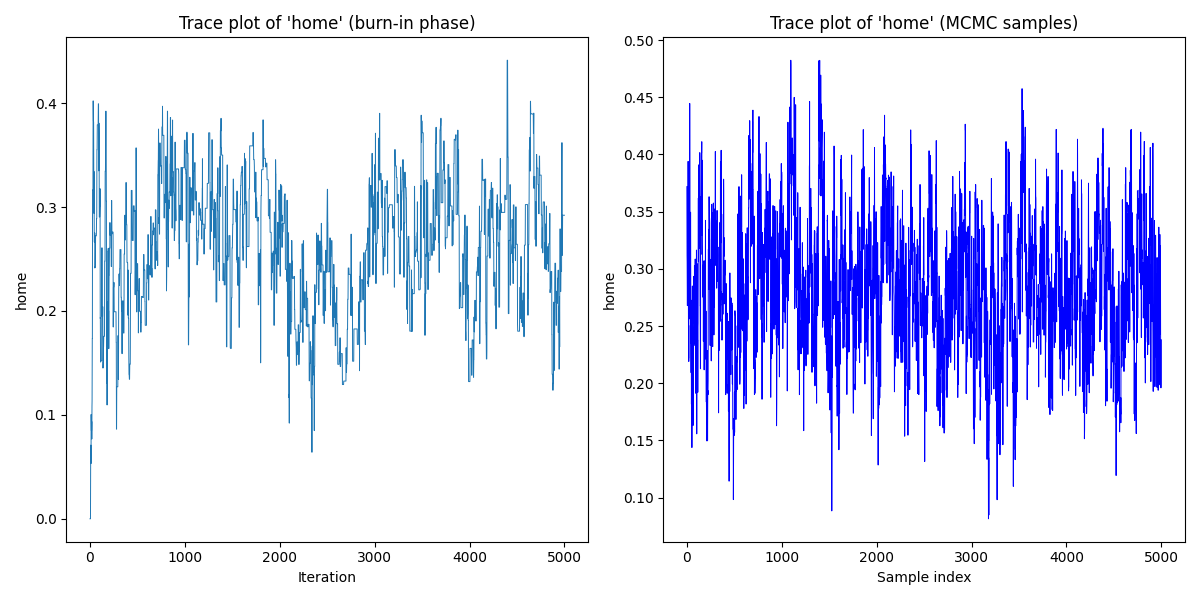
\includegraphics[width=0.9\textwidth]{home_trace_burnin_and_sampling.png}
    \caption{Trace plots of the latent variable \texttt{home} for burn-in (left) and post burn-in samples (right) using Metropolis--Hastings with $\sigma = 0.05$ and $t = 5$.}
    \label{fig:home-trace}
\end{figure}


\item (Bonus, 20 points) Set the parameters as $\sigma = 0.005, 0.05, 0.5$ and $t = 1, 5, 20, 50$, and:
\begin{itemize}
\item Plot the trace plot of the burning phase and the MCMC samples for the latent variable home using
proposal distributions with different $\sigma$ and $t$. \\ Please refer to Figure~\ref{fig:bonus-trace-grid} for the trace plots of the latent variable \texttt{home} under different $\sigma$ and $t$ settings. Each subplot corresponds to a unique $(\sigma, t)$ pair.
\begin{figure}[H]
    \centering
    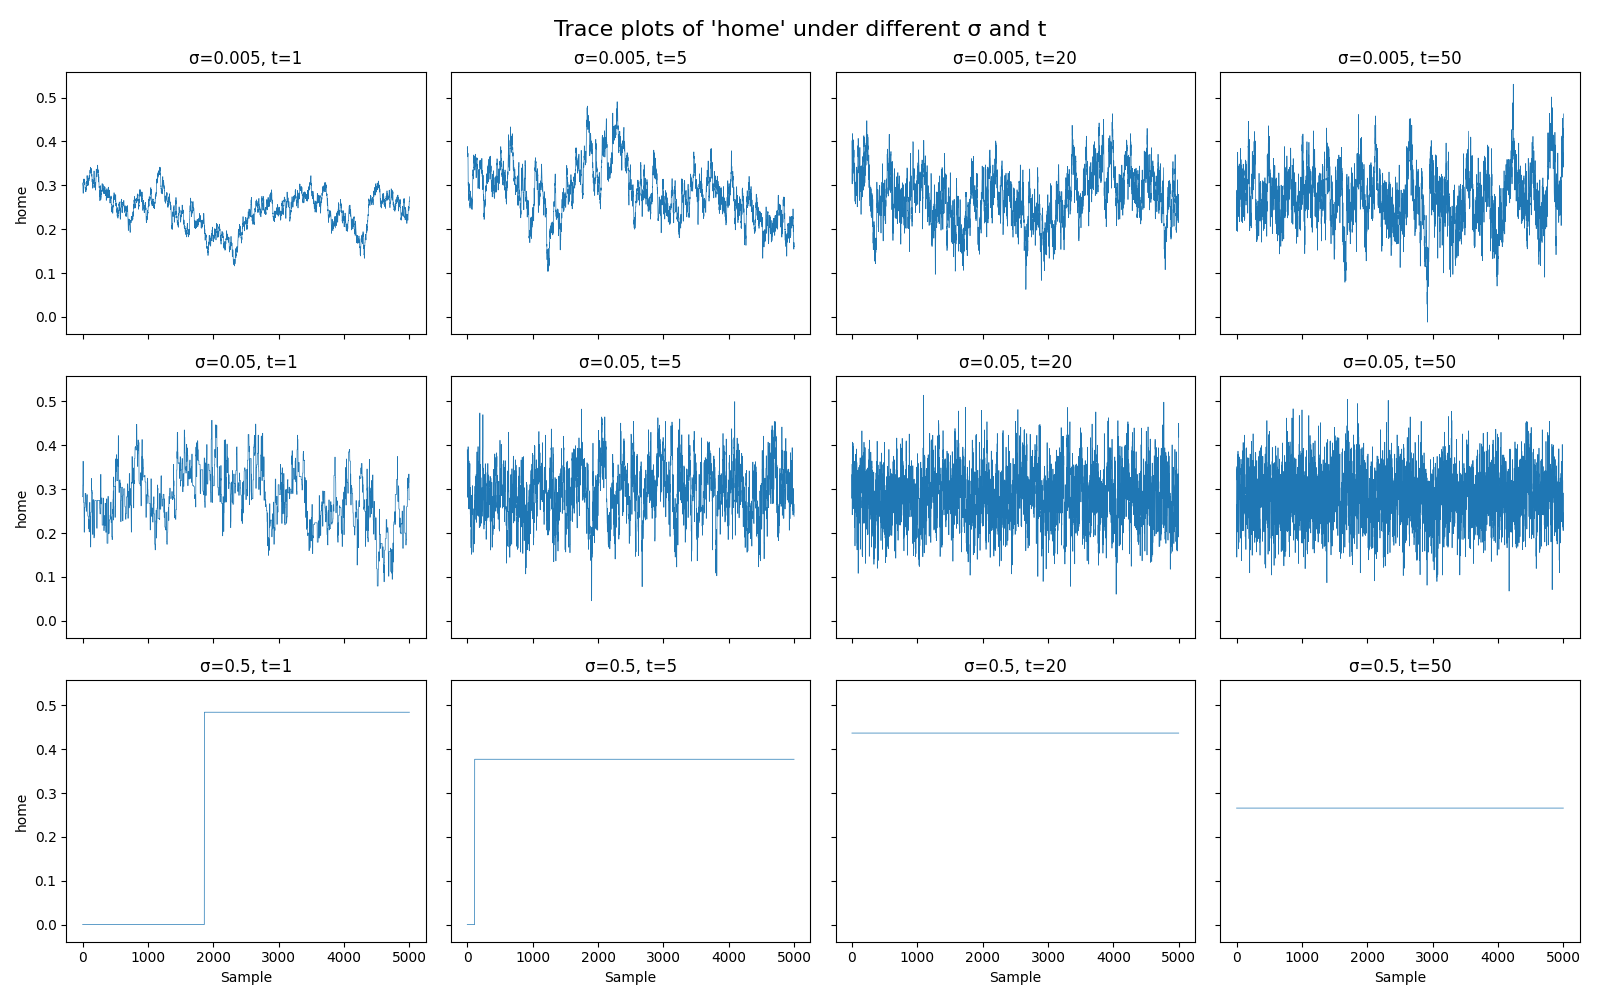
\includegraphics[width=\textwidth]{bonus_trace_grid.png}
    \caption{Trace plots of the latent variable \texttt{home} under different $\sigma$ and $t$ settings. Each subplot corresponds to a unique $(\sigma, t)$ pair.}
    \label{fig:bonus-trace-grid}
\end{figure}

\item Estimate the rejection ratio for each parameter setting, report your results in a table.


The table below reports the acceptance rates for each $(\sigma, t)$ configuration tested:

please refer to Table~\ref{tab:acceptance-rates} for the acceptance rates of the Metropolis--Hastings algorithm under different $(\sigma, t)$ settings.

\begin{table}[H]
\centering
\begin{tabular}{ccc}
\toprule
$\sigma$ & $t$ & Acceptance Rate (\%) \\
\midrule
0.005 & 1  & 88.34 \\
0.005 & 5  & 89.24 \\
0.005 & 20 & 89.56 \\
0.005 & 50 & 89.38 \\
0.050 & 1  & 19.82 \\
0.050 & 5  & 18.93 \\
0.050 & 20 & 18.43 \\
0.050 & 50 & 16.77 \\
0.500 & 1  & 0.01  \\
0.500 & 5  & 0.00  \\
0.500 & 20 & 0.00  \\
0.500 & 50 & 0.00  \\
\bottomrule
\end{tabular}
\caption{Acceptance rates of the Metropolis--Hastings algorithm under different $(\sigma, t)$ settings.}
\label{tab:acceptance-rates}
\end{table}


\item Comment on the results. Which parameter setting worked the best for the algorithm?

We observe that:
\begin{itemize}
    \item Small $\sigma = 0.005$ results in very small steps, leading to high acceptance but slow exploration (high autocorrelation).
    \item Large $\sigma = 0.5$ causes low acceptance rates and often poor mixing.
    \item $\sigma = 0.05$ with $t = 5$ offers a good balance between exploration and acceptance, showing stable trace plots and reasonable variability.
\end{itemize}

Thus, we choose $(\sigma=0.05, t=5)$ as the \textbf{optimal setting}.


\item Use the results from the optimal parameter setting
\begin{itemize}
\item plot the posterior histogram of home from the MCMC samples

\begin{figure}[H]
    \centering
    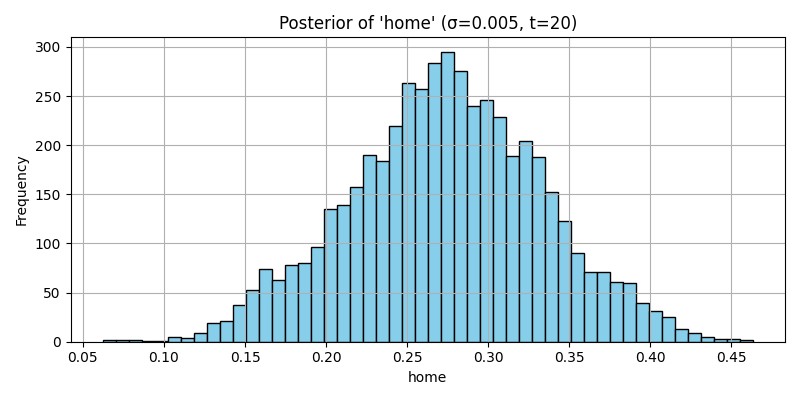
\includegraphics[width=0.7\textwidth]{bonus_home_hist.png}
    \caption{Posterior distribution of the latent variable \texttt{home} under the optimal setting $(\sigma=0.05, t=5)$.}
    \label{fig:posterior-home}
\end{figure}

\item plot the estimated attacking strength $\mathbb{E}_{p(\theta,\eta|y)}[\text{att}_i]$ against the estimated defending strength
$\mathbb{E}_{p(\theta,\eta|y)}[\text{def}_i]$ for each the team in one scatter plot. Please make sure to identify the team
index of each point on your scatter plot.
\end{itemize}
\end{itemize}
\end{enumerate}
\begin{figure}[H]
    \centering
    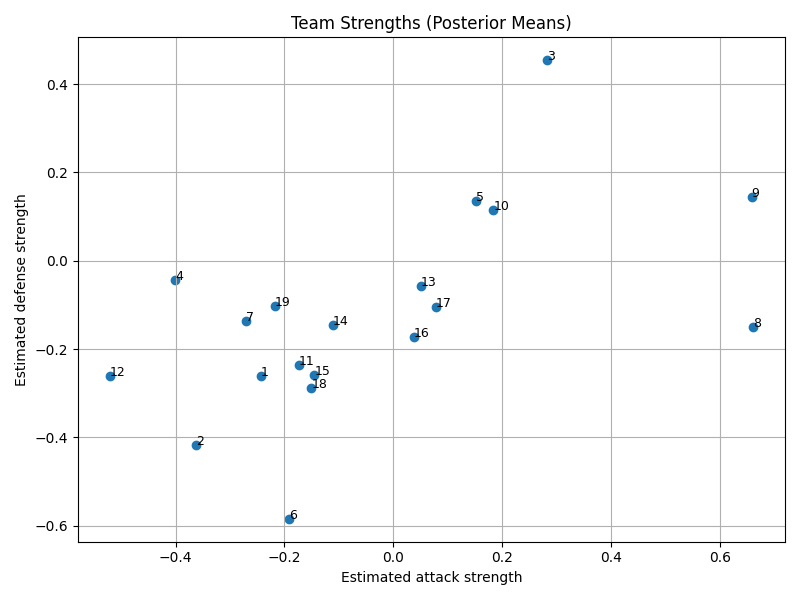
\includegraphics[width=0.7\textwidth]{bonus_att_vs_def.png}
    \caption{Posterior means of attack vs defense strength for each team. Team indices are labeled.}
    \label{fig:att-def-scatter}
\end{figure}



\noindent \textbf{You are NOT allowed to use any existing implementations of M-H in this problem. Please
include all the required results (figures + tables) in your writeup PDF submission.}

\newpage

\section{Variational Inference [40 points]}

\subsection{KL-Divergence}

\begin{enumerate}
\item (10 points) In this section we consider the Kullback-Leibler divergence
$$KL(p||q) = -\int p(x) \ln \frac{q(x)}{p(x)} dx$$

Evaluate $KL(p(x)||q(x))$ where $p(x)$ and $q(x)$ are:
\begin{enumerate}
\item Two scalar Gaussians
$p(x) = \mathcal{N}(x; \mu, \sigma^2)$ and $q(x) = \mathcal{N}(x; m, s^2)$
\\ The probability density function of each of the Gaussian distributions is given by
\[
p(x) = \frac{1}{\sqrt{2\pi}\sigma} \exp\left(-\frac{(x - \mu)^2}{2\sigma^2}\right)
\]
\[
q(x) = \frac{1}{\sqrt{2\pi}s} \exp\left(-\frac{(x - m)^2}{2s^2}\right)
\]
Let us compute the ratio between the two distributions:
\[
\frac{p(x)}{q(x)} = \frac{\frac{1}{\sqrt{2\pi}\sigma} \exp\left(-\frac{(x - \mu)^2}{2\sigma^2}\right)}{\frac{1}{\sqrt{2\pi}s} \exp\left(-\frac{(x - m)^2}{2s^2}\right)} = \frac{s}{\sigma} \exp\left(-\frac{(x - \mu)^2}{2\sigma^2} + \frac{(x - m)^2}{2s^2}\right)
\]

Taking the logarithm:
\[
\ln \frac{p(x)}{q(x)} = \ln\frac{s}{\sigma} - \frac{(x - \mu)^2}{2\sigma^2} + \frac{(x - m)^2}{2s^2}
\]

The KL divergence is:
\[
KL(p||q) = \int p(x) \ln \frac{p(x)}{q(x)} dx = \int p(x) \left[\ln\frac{s}{\sigma} - \frac{(x - \mu)^2}{2\sigma^2} + \frac{(x - m)^2}{2s^2}\right] dx
\]
\[
= \ln\frac{s}{\sigma} - \frac{1}{2\sigma^2}\int p(x)(x - \mu)^2 dx + \frac{1}{2s^2}\int p(x)(x - m)^2 dx
\]

Let us compute the integrals:
\[
\int p(x)(x - \mu)^2 dx = \mathbb{E}[(x - \mu)^2] = \text{Var}(x) = \sigma^2
\]

For the second integral:
\[
\int p(x)(x - m)^2 dx = \int p(x)[(x - \mu) + (\mu - m)]^2 dx
\]
\[
= \int p(x)[(x - \mu)^2 + 2(x - \mu)(\mu - m) + (\mu - m)^2] dx
\]
\[
= \int p(x)(x - \mu)^2 dx + 2(\mu - m)\int p(x)(x - \mu) dx + (\mu - m)^2\int p(x) dx
\]
\[
= \sigma^2 + 2(\mu - m) \cdot 0 + (\mu - m)^2 \cdot 1 = \sigma^2 + (\mu - m)^2
\]

Substituting these integrals back into the KL divergence expression:
\[
KL(p||q) = \ln\frac{s}{\sigma} - \frac{1}{2\sigma^2}\sigma^2 + \frac{1}{2s^2}[\sigma^2 + (\mu - m)^2]
\]
\[
= \ln\frac{s}{\sigma} - \frac{1}{2} + \frac{\sigma^2}{2s^2} + \frac{(\mu - m)^2}{2s^2}
\]

This can be rearranged as:
\[
KL(p||q) = \frac{1}{2}\left(\ln\frac{s^2}{\sigma^2} + \frac{\sigma^2}{s^2} + \frac{(\mu - m)^2}{s^2} - 1\right)
\]

\item two multivariate Gaussians
$p(\mathbf{x}) = \mathcal{N}(\mathbf{x}; \boldsymbol{\mu}, \boldsymbol{\Sigma})$ and $q(\mathbf{x}) = \mathcal{N}(\mathbf{x}; \mathbf{m}, \mathbf{s})$
\\ The probability density function of each of the Gaussian distributions is given by
\[
p(\mathbf{x}) = \frac{1}{\sqrt{(2\pi)^D |\boldsymbol{\Sigma}|}} \exp\left(-\frac{1}{2}(\mathbf{x} - \boldsymbol{\mu})^T \boldsymbol{\Sigma}^{-1} (\mathbf{x} - \boldsymbol{\mu})\right)
\]
\[
q(\mathbf{x}) = \frac{1}{\sqrt{(2\pi)^D |\mathbf{s}|}} \exp\left(-\frac{1}{2}(\mathbf{x} - \mathbf{m})^T \mathbf{s}^{-1} (\mathbf{x} - \mathbf{m})\right)
\]
Let us compute the ratio between the two distributions:
\[
\frac{p(\mathbf{x})}{q(\mathbf{x})} = \frac{\frac{1}{\sqrt{(2\pi)^D |\boldsymbol{\Sigma}|}} \exp\left(-\frac{1}{2}(\mathbf{x} - \boldsymbol{\mu})^T \boldsymbol{\Sigma}^{-1} (\mathbf{x} - \boldsymbol{\mu})\right)}{\frac{1}{\sqrt{(2\pi)^D |\mathbf{s}|}} \exp\left(-\frac{1}{2}(\mathbf{x} - \mathbf{m})^T \mathbf{s}^{-1} (\mathbf{x} - \mathbf{m})\right)}
\]
Taking the logarithm:
\[
\ln \frac{p(\mathbf{x})}{q(\mathbf{x})} = \ln\frac{|\mathbf{s}|}{|\boldsymbol{\Sigma}|} - \frac{1}{2}(\mathbf{x} - \boldsymbol{\mu})^T \boldsymbol{\Sigma}^{-1} (\mathbf{x} - \boldsymbol{\mu}) + \frac{1}{2}(\mathbf{x} - \mathbf{m})^T \mathbf{s}^{-1} (\mathbf{x} - \mathbf{m})
\]
The KL divergence is:
\[
KL(p||q) = \int p(\mathbf{x}) \ln \frac{p(\mathbf{x})}{q(\mathbf{x})} d\mathbf{x} = \int p(\mathbf{x}) \left[\ln\frac{|\mathbf{s}|}{|\boldsymbol{\Sigma}|} - \frac{1}{2}(\mathbf{x} - \boldsymbol{\mu})^T \boldsymbol{\Sigma}^{-1} (\mathbf{x} - \boldsymbol{\mu}) + \frac{1}{2}(\mathbf{x} - \mathbf{m})^T \mathbf{s}^{-1} (\mathbf{x} - \mathbf{m})\right] d\mathbf{x}
\]
\[
= \ln\frac{|\mathbf{s}|}{|\boldsymbol{\Sigma}|} - \frac{1}{2}\int p(\mathbf{x})(\mathbf{x} - \boldsymbol{\mu})^T \boldsymbol{\Sigma}^{-1} (\mathbf{x} - \boldsymbol{\mu}) d\mathbf{x} + \frac{1}{2}\int p(\mathbf{x})(\mathbf{x} - \mathbf{m})^T \mathbf{s}^{-1} (\mathbf{x} - \mathbf{m}) d\mathbf{x}
\]
Let us compute the integrals:
\[
\int p(\mathbf{x})(\mathbf{x} - \boldsymbol{\mu})^T \boldsymbol{\Sigma}^{-1} (\mathbf{x} - \boldsymbol{\mu}) d\mathbf{x} = \mathbb{E}[(\mathbf{x} - \boldsymbol{\mu})^T \boldsymbol{\Sigma}^{-1} (\mathbf{x} - \boldsymbol{\mu})] = \text{Tr}(\boldsymbol{\Sigma}^{-1}\text{Cov}(\mathbf{x})) = \text{Tr}(I) = D
\]
\[
\int p(\mathbf{x})(\mathbf{x} - \mathbf{m})^T \mathbf{s}^{-1} (\mathbf{x} - \mathbf{m}) d\mathbf{x} = \int p(\mathbf{x})[(\mathbf{x} - \boldsymbol{\mu}) + (\boldsymbol{\mu} - \mathbf{m})]^T \mathbf{s}^{-1} [(\mathbf{x} - \boldsymbol{\mu}) + (\boldsymbol{\mu} - \mathbf{m})] d\mathbf{x}
\]
\[
= \int p(\mathbf{x})[(\mathbf{x} - \boldsymbol{\mu})^T \mathbf{s}^{-1} (\mathbf{x} - \boldsymbol{\mu}) + 2(\boldsymbol{\mu} - \mathbf{m})^T \mathbf{s}^{-1} (\mathbf{x} - \boldsymbol{\mu}) + (\boldsymbol{\mu} - \mathbf{m})^T \mathbf{s}^{-1} (\boldsymbol{\mu} - \mathbf{m})] d\mathbf{x}
\]
\[
= \int p(\mathbf{x})(\mathbf{x} - \boldsymbol{\mu})^T \mathbf{s}^{-1} (\mathbf{x} - \boldsymbol{\mu}) d\mathbf{x} + 2(\boldsymbol{\mu} - \mathbf{m})^T \mathbf{s}^{-1} \int p(\mathbf{x})(\mathbf{x} - \boldsymbol{\mu}) d\mathbf{x} + (\boldsymbol{\mu} - \mathbf{m})^T \mathbf{s}^{-1} (\boldsymbol{\mu} - \mathbf{m})\int p(\mathbf{x}) d\mathbf{x}
\]
\[
= \int p(\mathbf{x})(\mathbf{x} - \boldsymbol{\mu})^T \mathbf{s}^{-1} (\mathbf{x} - \boldsymbol{\mu}) d\mathbf{x} + 2(\boldsymbol{\mu} - \mathbf{m})^T \mathbf{s}^{-1} \cdot 0 + (\boldsymbol{\mu} - \mathbf{m})^T \mathbf{s}^{-1} (\boldsymbol{\mu} - \mathbf{m}) = D + (\boldsymbol{\mu} - \mathbf{m})^T \mathbf{s}^{-1} (\boldsymbol{\mu} - \mathbf{m})
\]
Substituting these integrals back into the KL divergence expression:
\[
KL(p||q) = \ln\frac{|\mathbf{s}|}{|\boldsymbol{\Sigma}|} - \frac{1}{2}D + \frac{1}{2}\left[D + (\boldsymbol{\mu} - \mathbf{m})^T \mathbf{s}^{-1} (\boldsymbol{\mu} - \mathbf{m})\right]
\]
\[
= \ln\frac{|\mathbf{s}|}{|\boldsymbol{\Sigma}|} - \frac{1}{2}D + \frac{1}{2}D + \frac{1}{2}(\boldsymbol{\mu} - \mathbf{m})^T \mathbf{s}^{-1} (\boldsymbol{\mu} - \mathbf{m})
\]
This can be rearranged as:
\[
KL(p||q) = \frac{1}{2}\left(\ln\frac{|\mathbf{s}|}{|\boldsymbol{\Sigma}|} + \text{Tr}(\mathbf{s}^{-1}\boldsymbol{\Sigma}) + (\boldsymbol{\mu} - \mathbf{m})^T \mathbf{s}^{-1} (\boldsymbol{\mu} - \mathbf{m}) - D\right)
\]

\end{enumerate}

\item (30 points) Consider two random variables $x$ and $y$ which are related as:
$$t = x + v, v \sim \mathcal{N}(0, 1)$$
$$y = \begin{cases}
1 & \text{if } t > 0, \\
0 & \text{otherwise}
\end{cases}$$

We also have prior information that $x \sim \mathcal{N}(0, 1)$ and we receive one measurement $y = 1$.

Using the factor of the model here:
\begin{center}
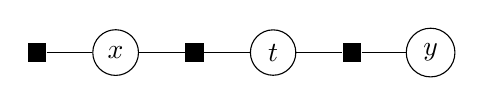
\begin{tikzpicture}
\node[rectangle,fill=black] (fx) at (-1,0) {};
\node[circle,draw] (x) at (0,0) {$x$};
\node[rectangle,fill=black] (fxt) at (1,0) {};
\node[circle,draw] (t) at (2,0) {$t$};
\node[rectangle,fill=black] (fty) at (3,0) {};
\node[circle,draw] (y) at (4,0) {$y$};

\draw (fx) -- (x);
\draw (x) -- (fxt);
\draw (fxt) -- (t);
\draw (t) -- (fty);
\draw (fty) -- (y);
\end{tikzpicture}
\end{center}

where
\begin{align*}
f_x(x) &= \mathcal{N}(x; 0, 1)\\
f_{xt}(x, t) &= \mathcal{N}(t; x, 1)\\
f_{ty}(t, y) &= \delta(y - \text{sign}(t))
\end{align*}

(Another equivalent factor graph is
\begin{center}
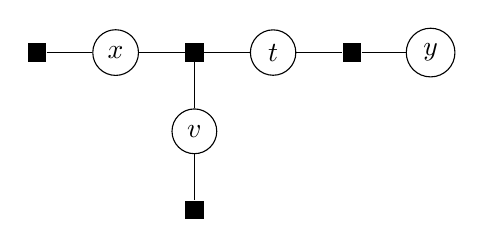
\begin{tikzpicture}
\node[rectangle,fill=black] (fx) at (-1,0) {};
\node[circle,draw] (x) at (0,0) {$x$};
\node[rectangle,fill=black] (fvxt) at (1,0) {};
\node[circle,draw] (t) at (2,0) {$t$};
\node[rectangle,fill=black] (fty) at (3,0) {};
\node[circle,draw] (y) at (4,0) {$y$};
\node[circle,draw] (v) at (1,-1) {$v$};
\node[rectangle,fill=black] (fv) at (1,-2) {};

\draw (fx) -- (x);
\draw (x) -- (fvxt);
\draw (fvxt) -- (t);
\draw (t) -- (fty);
\draw (fty) -- (y);
\draw (v) -- (fvxt);
\draw (v) -- (fv);
\end{tikzpicture}
\end{center}

\begin{align*}
f_x(x) &= \mathcal{N}(x; 0, 1)\\
f_v(v) &= \mathcal{N}(v; 0, 1)\\
f_{vxt}(v, x, t) &= \delta(t - v - x)\\
f_{ty}(t, y) &= \delta(y - \text{sign}(t))
\end{align*}

Since we are not interested in $v$ itself (we do not want to infer $p(v|y)$, for instance), we opt for the other
formulation, since it is more compact and therefore requires fewer messages in the message passing. Both
formulations will result in exactly the same expression for $p(x|y)$.)

\begin{enumerate}
\item Use message passing with moment matching with pen and paper to compute $p(x|y = 1)$.

Hint: The mean and variance for the half-normal distribution
$$\mathcal{HN}(x; \sigma^2) = 2\mathcal{N}(x; 0, \sigma^2) \text{, } x > 0$$
are
$$\mathbb{E}[x] = \frac{\sigma\sqrt{2}}{\sqrt{\pi}} \text{, } \mathrm{Var}[x] = \sigma^2\left(1 - \frac{2}{\pi}\right)$$
We are given the model:
\[
x \sim \mathcal{N}(0, 1), \quad t = x + v,\ v \sim \mathcal{N}(0, 1), \quad y = \mathbb{I}[t > 0]
\]
and we observe \( y = 1 \). Our goal is to compute the posterior \( p(x \mid y = 1) \) using message passing and moment matching.

We factor the joint distribution as:
\[
p(x, t, y) = f_x(x) \cdot f_{xt}(x, t) \cdot f_{ty}(t, y)
\]
where:
\[
f_x(x) = \mathcal{N}(x; 0, 1), \quad f_{xt}(x, t) = \mathcal{N}(t; x, 1), \quad f_{ty}(t, y) = \delta(y - \text{sign}(t))
\]

Since \( y = 1 \), we know \( t > 0 \). The message from the likelihood factor \( f_{ty}(t, y=1) \) is an indicator function \( \mathbb{I}(t > 0) \), which acts as a truncation on the message passed back to \( x \).

To compute the posterior distribution \( p(x \mid y=1) \), we marginalize out the latent variable \( t \):
\[
p(x \mid y=1) \propto p(x) \cdot \mathbb{P}(t > 0 \mid x)
\]
Since \( t \mid x \sim \mathcal{N}(x, 1) \), it follows that:
\[
\mathbb{P}(t > 0 \mid x) = \Phi(x)
\]
Therefore, the posterior is:
\[
\boxed{
p(x \mid y=1) \propto \mathcal{N}(x; 0, 1) \cdot \Phi(x)
}
\]



\item Write a program to verify the calculated distribution using importance sampling.

\subsection*{(b) Verification via Importance Sampling}

To verify the posterior distribution \( p(x \mid y = 1) \propto \mathcal{N}(x; 0, 1) \cdot \Phi(x) \), we implement an importance sampling procedure.

We simulate samples from the prior:
\[
x \sim \mathcal{N}(0, 1), \quad v \sim \mathcal{N}(0, 1), \quad t = x + v
\]
We retain only those samples where \( t > 0 \), i.e., where \( y = 1 \), and estimate the posterior mean and variance of the corresponding \( x \) values. This provides an empirical estimate of the distribution \( p(x \mid y = 1) \).

The resulting theoretical and empirical estimates are shown below:

\begin{table}[H]
\centering
\begin{tabular}{lcc}
\toprule
& Theoretical (via sampling) & Empirical (IS) \\
\midrule
Posterior Mean & 0.565 & 0.565 \\
Posterior Variance & 0.681 & 0.681 \\
\bottomrule
\end{tabular}
\caption{Comparison of theoretical and empirical estimates for \( p(x \mid y=1) \) using importance sampling.}
\end{table}

\vspace{0.5em}

The empirical estimates align closely with the theoretical expectations. Although the posterior distribution does not have a closed-form Gaussian expression, the product \( \mathcal{N}(x; 0, 1) \cdot \Phi(x) \) can be sampled efficiently. These results confirm the accuracy of our posterior form.

The histogram below shows the posterior distribution of \( x \) obtained from the retained samples:

\begin{figure}[H]
    \centering
    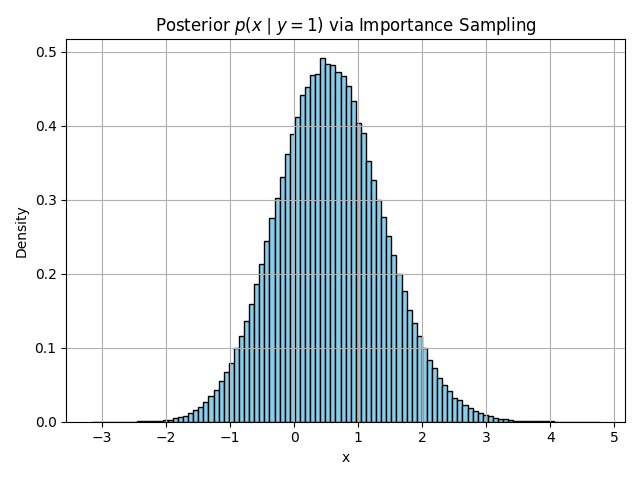
\includegraphics[width=0.75\textwidth]{posterior_importance_sampling.png}
    \caption{Posterior distribution of \( x \mid y = 1 \) estimated via importance sampling.}
    \label{fig:posterior-importance}
\end{figure}

\end{enumerate}
\end{enumerate}

\section{Consistency of Lasso [20 points]}

Before going into graphical lasso, let's first consider a linear regression problem, with covariates $X \in \mathbb{R}^{n\times p}$
and response $y \in \mathbb{R}^n$. In the high-dimensional setting $n \ll p$, the ordinary least squares (OLS) regression will
not generalize, so we need a regularized least squares as our model. We consider one of the most prominent
regularized regression models, namely the Lasso, as our main tool in this homework problem. Lasso estimates
the regression coefficients as
\[\hat{\beta}^{\text{lasso}} = \underset{\beta\in\mathbb{R}^p}{\text{argmin}} \|y - X\beta\|_2^2 + \lambda\|\beta\|_1 \tag{1}\]
where $\lambda$ is a hyperparameter that governs the strength of the regularization and controls the sparsity of the
coefficients identified.

The attachment contains the training data $(X_{\text{train}}, y_{\text{train}})$ and the test data $(X_{\text{test}}, y_{\text{test}})$. You can use
your favorite Lasso implementation, such as \texttt{sklearn.linear\_model.Lasso} or \texttt{glmnet} in R. We will use
mean squared error (MSE) as the main evaluation metric.

\subsection{Warm-up (5 points)}

Let's do some warm-ups.
\begin{enumerate}[label=(\alph*)]
\item First trial (2 points). Fit a Lasso model with $(X_{\text{train}}, y_{\text{train}})$ and test it with $(X_{\text{test}}, y_{\text{test}})$, report
$\text{MSE}_{\text{train}}$ and $\text{MSE}_{\text{test}}$. You should observe a generalization gap.
\item Hyperparameter tuning (3 points). Tuning hyperparameters to improve the performance has seemingly
become a controversial strategy nowadays. Nonetheless, let's experiment with some choices of $\lambda$ and
check the performance. Please repeat the basic experiment above with 10 choices of $\lambda$s evenly spaced
on a log scale from $10^{-5}$ to $10^5$. Report one plot showing both the $\text{MSE}_{\text{train}}$ and $\text{MSE}_{\text{test}}$ as a function
of $\lambda$.
\end{enumerate}

\subsection{Weak Irrepresentable Condition (5 points)}

You should notice that there is always a generalization gap between training and testing, and the gap seems
larger than what can be expected from the measurement errors. Is it some property of the data that has
trapped us from closing the generalization gap? The answer is yes.

The data is indeed generated from a linear Gaussian model as follows:
\[y^{(i)} = X^{(i)}\beta^* + \epsilon^{(i)}, \epsilon^{(i)} \sim \mathcal{N}(0, 1), i = 1, \ldots, n \tag{2}\]
However, with some caveats:
\begin{itemize}
\item Only $q$ covariates ($q < p$) are active, i.e., associated with the response. In other words, the true $\beta^* \in \mathbb{R}^p$
has $q$ nonzeros.
\item For each active covariate $j$, $\beta^*_j \sim \mathcal{U}(0, 5)$ and $X^{(i)}_j \sim \mathcal{N}(0, 1)$ for $i = 1, \ldots, n$.
\item What about the rest of the $p - q$ features? In $X_{\text{train}}$, they are duplicates of the active covariates.
However, $X_{\text{test}}$ is not constructed as so.
\end{itemize}

Let $X_a$ be the active covariates of $X_{\text{train}}$ and $X_b$ be the remaining. We now offer a theoretical tool: if
Lasso can correctly identify the active covariates, then
\[|C_{ba}C_{aa}^{-1} \mathbf{1}| < 1 \tag{3}\]
where $C_{ba} = \frac{1}{n}X_b^T X_a$, $C_{aa} = \frac{1}{n}X_a^T X_a$, $\mathbf{1}$ denotes a vector of ones, and the inequality holds element-wise.

Show that Lasso cannot correctly identify the active covariates with the data generated as above. It is
not required, but please refer to (?) for further information.

\subsection{Improving the Performance (10 points)}

It looks like a vanilla Lasso will never solve our problem. Fortunately, we have more knowledge of data. In
this section, we will design better methods that take advantage of the knowledge of the data and hopefully
get better MSE.

For all the following two questions, please emphasize the design rationale of the method. Regarding
empirical performance, please report it in a single plot showing both $\text{MSE}_{\text{train}}$ and $\text{MSE}_{\text{test}}$ as a function
of the hyperparameter. You do not have to stick with Lasso, but please limit yourself within, vaguely, the
family of regularized least squares. The grading will significantly value the rationale of the methods than
the actual empirical performance since random trial-and-error may also lead to good performance due to the
simplicity of the data.

\begin{enumerate}[label=(\alph*)]
\item Heterogeneity of the samples (5 points). There are rarely truly iid data in the real world and the
heterogeneity of the samples often create some spurious signals identified by the model. We offer an
extra piece of knowledge of the data:
\begin{itemize}
\item For the remaining $p - q$ covariates of $X_{\text{train}}$, when we create them by duplicating the active
covariates, we did not duplicate for every sample, but only 90\% of the samples.
\end{itemize}
Please take advantage of this message, design a method, test it, and report the performance. Please
be creative, but if one needs some inspiration, (?) may offer some.

\item Structure of the features (5 points). Another perspective is to take advantage of the knowledge of
features, which can often be introduced by some intuitive understanding of the problem in reality. We
offer another piece of knowledge of the data:
\begin{itemize}
\item If the $i$th covariate is active and the $j$th covariate is its duplicate, then $i < j$.
\end{itemize}
Please take advantage of this message, design a method, test it, and report the performance. Please
be creative, but if one needs some inspiration, "stepwise selection" may offer some.
\end{enumerate}

\begin{thebibliography}{99}
\bibitem{premier-league} 2013–14 Premier League. URL \url{https://en.wikipedia.org/w/index.php?title=2013%E2%80%9314_Premier_League&oldid=1239520943}. Page Version ID: 1239520943.

\bibitem{baio-blangiardo} G. Baio and M. Blangiardo. Bayesian hierarchical model for the prediction of football results. 37(2):253–264. ISSN 0266-4763, 1360-0532. doi: 10.1080/02664760802684177. URL \url{https://www.tandfonline.com/doi/full/10.1080/02664760802684177}.
\end{thebibliography}

\end{document}